\documentclass[12pt]{article}
	
%______________________PREAMBULO_________________________

%----------------------Paquetes--------------------------
\usepackage{amsmath,amssymb,amsfonts,latexsym,cancel} % Paquetes de símbolos adicionales.
\usepackage[spanish,es-tabla]{babel} % Idioma español
\usepackage[utf8]{inputenc} % Paquete que nos permite usar los acentos y otros símbolos, directamente del teclado.
\usepackage[T1]{fontenc} % Cambia el tipo de letra
\usepackage{times} % Tipo de letra Times New Roman
\usepackage{graphicx} % Paquete para el manejo de gráficos y figuras en el documento.
\usepackage{geometry} % Permite el manejo de los margenes
\usepackage{fancyhdr} % Permite colocar y manejar el encabezado
\usepackage[breaklinks,colorlinks=true,linkcolor=black,citecolor=blue, urlcolor=blue]{hyperref} % Crea hipervinculo entre secciones y el indice
\usepackage{pstricks}
\usepackage{multicol}
%\usepackage{mathpazo} %fuente palatino
%\usepackage{xcolor}
%\usepackage[shortlabels]{enumitem}
%-------------Paquetes para el formato de las citas-------
%\usepackage[hyphens]{url}
%\usepackage{float}
%\usepackage{cite}
%\usepackage{wrapfig}

%-----------------------------ayuda de paquetes--------------------

\spanishdecimal{.}

%------------------------Margenes----------------------------

\newgeometry{bottom = 2.5 cm, top = 2.5 cm, left = 2 cm, right = 2 cm} % Modifica el margen {Abajo, Arriba, Izquierda, Derecha

%----------------------------Interlineado----------------------------------

%\doublespacing
%\onehalfspace
%\singlespace
%\spacing{1.5} % Permite personalisar a gusto
%\setlength{\parskip}{2cm} % Es el espacio entre parrafos

%-----------------------------Sangria---------------------------------------

\setlength{\parindent}{0 cm} % Manipula la sangria

%---------------------Portada------------------

%\title{
%\begin{figure}[h!]
		
%	\centering
%	
\includegraphics[width=\linewidth]{Nom_UAdeC_FCFM.png}  			
			
%\end{figure}
%\huge \textbf{LABORATORIO DE FISICA 3}\\\LARGE TITULO PRACTICA\\}
%\author{ \Large \textbf{Profesor:}\\
%\Large \textbf{Alumno:} Oscar Joel Castro Contreras}
%\date{\today}

%--------------Encabezado y pie de pagina--------------------

\pagestyle{fancy}%Coloca el encabezado en el documento
\lhead[]{Métodos numéricos}%Encabezado izquierda
\rhead[]{Oscar Joel Castro Contreras}%Encabesado derecha
%\chead[]{}%Encabesado central
\renewcommand{\headrulewidth}{0.08 pt}%Coloca linea al pie de pagina

%\lfoot[]{PI}%Pie de pagina izquerdo
%\rfoot[]{PD}%Pie de pagina derecho
\cfoot[]{\thepage}%Pie de pagina central
\renewcommand{\footrulewidth}{0.08 pt}%Coloca linea al pie de pagina

%-----------------------------------------------------------------------------

	\begin{document}
		
		\begin{titlepage}
		
			\centering
			{\bfseries
			\begin{figure}[h!]
				\centering
				
\includegraphics[width=\linewidth]{Nom_UAdeC_FCFM.png} 				
			\end{figure}
			\par}
			\vspace{2cm}
			{\scshape\LARGE Métodos numéricos \par}
			\vspace{3cm}
			{\scshape\Huge \textbf{Método de Gauss Siedel} \par}
			\vfill
			{\LARGE \textbf{Profesora:} Maria Guadalupe Godina Cubillo \par}
			\vspace{3cm}
			{\LARGE \textbf{Alumno:} Oscar Joel Castro Contreras \par}
			\vfill
			{\Large \today \par}
			\thispagestyle{empty}
			%\thispagestyle{fancy}
			
		\end{titlepage}
	
		\newpage

		\begin{abstract}
			\noindent En este reporte explico un poco lo que es un método iterativo y en qué consisten. También explico 
			a detalle cual es el procedimiento que sigue el método de Gauss Seidel, doy algunos ejemplos y 
			explico cuáles son sus condiciones y las restricciones que tiene.
			
		\end{abstract}

          \textbf{Palabras clave:} Método iterativo, Método de Jacobi, Matriz diagonalmente dominante.

		\section*{\centering Introducción}\label{sec:Introducción}
			Los métodos iterativos se caracterizan por la sencillez de las operaciones asociadas y ser de fácil 
			implementación en ordenadores. Son relativamente insensibles a la propagación de errores. Cada 
			método iterativo, y a partir de una solución aproximada, genera una sucesión de soluciones que bajo 
			ciertas condiciones converge hacia la solución exacta. Son métodos preferibles a los directos para 
			sistemas de cientos de variables, particularmente si muchos de los coeficientes son nulos, como 
			ocurre en problemas numéricos asociados a ecuaciones en derivadas parciales. 
			Los métodos iterativos para sistemas lineales son una generalización del método del punto fijo para 
			obtener los ceros de una función no lineal. Dado el sistema lineal $ Ax = b $, donde $ A $ es una 
			matriz no singular, todo método iterativo para resolverlo está definido por una descomposición 
			particular $ A = M - N $, donde $ M $ es una matriz no singular fácilmente invertible. El sistema 
			lineal puede representarse como $ Mx = Nx + b $, de donde obtenemos $ x = M^{-1}Nx + M^{-1}b $. 
			De esta forma, obtenemos el sistema lineal equivalente al original $ x = Px + c $, siendo 
			$ P = M^{-1}N $ y $ c = M^{-1}b $ que tiene la forma apropiada para aplicar el método iterativo del
			punto fijo para el sistema lineal de ecuaciones: $$ x_{n+1} = Px_n + c $$ \cite{bib:item1}

		\section*{\centering Metodología}\label{sec:Metodologia}
			El método de Gauss seidel consiste en tener un sistema de ecuaciones $ Ax = b $,  donde $ A $ es una 
			matriz con un determinante distinto de cero y que sea invertible, por ejemplo:
			\begin{align*}
				a_{11}x_1 + a_{12}x_2 + a_{13}x_3 &= b_1 \\
				a_{21}x_1 + a_{22}x_2 + a_{23}x_3 &= b_2 \\
				a_{31}x_1 + a_{32}x_2 + a_{33}x_3 &= b_3
			\end{align*}
			Para entender de forma más fácil, si usamos este sistema de ecuaciones la que se haría es despeja 
			$ x_1 $ de la primera ecuación, $ x_2 $ de la segunda y $ x_ 3 $ de la tercera, así sucesivamente, 
			dependiendo de las ecuaciones que se tengan. Donde $ a_{11} $, $ a_{22} $ y $ a_{33} $, son distintos 
			de cero. entonces tendríamos algo como:
			\begin{align*}
				x_1 &= \frac{b_1 - a_{12}x_2 - a_{13}x_3}{a_{11}} \\
				x_2 &= \frac{b_2 - a_{21}x_1 - a_{23}x_3}{a_{22}} \\
				x_3 &= \frac{b_3 - a_{31}x_1 - a_{32}x_2}{a_{33}}
			\end{align*}
			Una ves que se tenga esto se da un valor inicial a cada variable, por lo que tendríamos un vector como:
			$$
			x^{(k)} =
			\left[\begin{array}{c}
				x_1^k \\
				x_2^k \\
				x_3^k 
			\end{array}\right]
			$$
			Donde en este método, los valores que se van calculando en la $(k+1)-$ésima iteración se emplean para 
			estimar los valores faltantes de esa misma iteración, es decir con $ x^{(k)} $ se calcula $ x^{(k+1)} $ 
			de acuerdo con
			$$
			x^{(k+1)} =
			\left[\begin{array}{c}
				x_1^{k+1} \\
				x_2^{k+1} \\
				x_3^{k+1} 
			\end{array}\right]
			=
			\left[\begin{array}{c}
				\frac{1}{a_{11}}(b_1 - a_{12}x_2^k - a_{13}x_3^k) \\
				\frac{1}{a_{22}}(b_2 - a_{21}x_1^{k+1} - a_{23}x_3^k) \\
				\frac{1}{a_{33}}(b_3 - a_{31}x_1^{k+1} - a_{32}x_2^{k+1})
			\end{array}\right]
			$$
			Entonces siguiendo esto ir iterando, el método convergerá cuando los valores de $ x^k $ se acerquen a la 
			solución del sistema, el criterio de paro esta dado por:
			$$ \parallel x^{k+1} – x^k \parallel < \epsilon $$
			Es cuando el valor absoluto de la resta de los vector $ x^{k+1} - x^k $ es menor un cierto número de cifras 
			significativas deseado $ (\epsilon) $.
			Pero hay mas condiciones para que este método converge como algunas ya dichas. La matriz que se forme 
			tenga un determinante distinto de cero, que esta matriz tenga inversa y que en la diagonal no haya ceros. Pero 
			aún hay mas condiciones, por ejemplo, este método también solo converge sin la matriz es diagonalmente dominante, 
			esto significa que la diagonal de la matriz cumple con:
			$$
			\begin{array}{c c c c c c}
				\mid a_{11} \mid & > & \mid a_{12} \mid + \mid a_{13} \mid & + \dots + & \mid a_{1n} \mid \\
				\mid a_{22} \mid & > & \mid a_{21} \mid + \mid a_{23} \mid & + \dots + & \mid a_{2n} \mid \\
				\vdots &  & \vdots & \ddots & \vdots \\
				\mid a_{nn} \mid & > & \mid a_{n1} \mid + \mid a_{n2} \mid & + \dots + & \mid a_{nn-1} \mid 
			\end{array}
			$$
			Si la matriz no cumple estas condiciones el método nunca converge, en contrario diverge.
			Pero como son muchas condiciones solo hay que enfocarnos en que sea diagonalmente domínate y que no tenga ceros 
			en la diagonal, si lo matriz cumple estos 2 criterios, todo los demás criterios automaticamente se cumplirán.

		\section*{\centering Resultado}\label{sec:Resultado}
			Si tomamos de ejemplo el sistema de ecuaciones siguiente:
			\begin{align*}
				3x_1 - 0.1x_2 - 0.2x_3 &= 7.85 \\
				0.1x_1 + 7x_2 - 0.3x_3 &= -19.3 \\
				0.3x_1 - 0.2x_2 + 10x_3 &= 71.4
			\end{align*}
			Y  si lo vemos de forma matricial seria:
			$$
			\left(\begin{array}{ccc}
				3 & -0.1 & -0.2 \\
				0.1 & 7 & -0.3 \\
				0.3 & -0.2 & 10
			\end{array}\right)
			\left(\begin{array}{c}
				x_1 \\
				x_2 \\
				x_3 
			\end{array}\right)
			   =
			\left(\begin{array}{c}
			 7.85 \\
			 -19.3 \\
			 71.4 
			\end{array}\right)
			$$
			Donde el resultado es $ x_1 = 3 $, $ x_2 = -2.5 $ y $ x_3 = 7 $.\\
			Ahora hay que ver que los criterios para este método se cumplan. El primero, la diagonal no puede tener ceros y 
			observando el sistema este criterio si se cumplen. El segundo, la diagonal de la matriz debe ser dominante, hacemos 
			los cálculos siguiendo lo explicado:
			$$
			\begin{array}{c c c c c c}
				\mid 3 \mid & > & \mid -0.1 \mid + \mid -0.2 \mid & = & 0.3 \\
				\mid 7 \mid & > & \mid 0.1 \mid + \mid -0.3 \mid & = & 0.4 \\
				\mid 10 \mid & > & \mid 0.3 \mid + \mid -0.2 \mid & = & 0.5 
			\end{array}
			$$
			Vemos que si se cumple por lo que ahora procedemos a despejar como se dijo anteriormente cada variable obteniendo:
			\begin{align*}
				x_1 &= \frac{7.85 + 0.1x_2 + 0.2x_3}{3} \\
				x_2 &= \frac{-19.3 - 0.1x_1 + 0.3x_3}{7} \\
				x_3 &= \frac{71.4 - 0.3x_1 + 0.2x_2}{10}
			\end{align*}
			Ahora tenemos que dar un valor inicial a cada variable lo más común es que se les dé un valor de cero, por lo que 
			el vector $ x^{(0)} $ seria
			$$
			x^{(0)} =
			\left[\begin{array}{c}
				0 \\
				0 \\
				0 
			\end{array}\right]
			$$
			Ahora hay que obtener lo que vale la primera variable $ x_1 $ sustituyendo lo valores iniciales que dimos entonces
			$$ x_1 = \frac{7.85 + 0.1(0) + 0.2(0)}{3} = 2.616667 $$
			Ahora hay que obtener lo que vale la segunda variable $ x_2 $ sustituyendo ahora con el valor de $ x_1 $ y los valores 
			iniciales dado de las otras variables entonces obtendríamos
			$$ x_2 = \frac{-19.3 - 0.1(2.616667) + 0.3/(0)}{7} = 2.794524 $$
			Seguimos ahora con la variable $ x_3 $, de igual forma sustituyendo los valores que se obtuvieron de las anteriores 
			variables, entonces tendríamos que
			$$ x_3 = \frac{71.4 - 0.3(2.616667) + 0.2(-2.794524)}{10} = 7.005610 $$
			Y así se ira iterando hasta obtener la solución del sistema, por lo que hay que realizar un programa de computadora para 
			realizar esto más rápido, si introduzco este sistema de ecuaciones en mi programa que realiza el procedimiento anterior y 
			tomando el criterio de paro que ya se menciono antes, obtengo lo que se puede ver en la figura 1.
			\begin{center}
				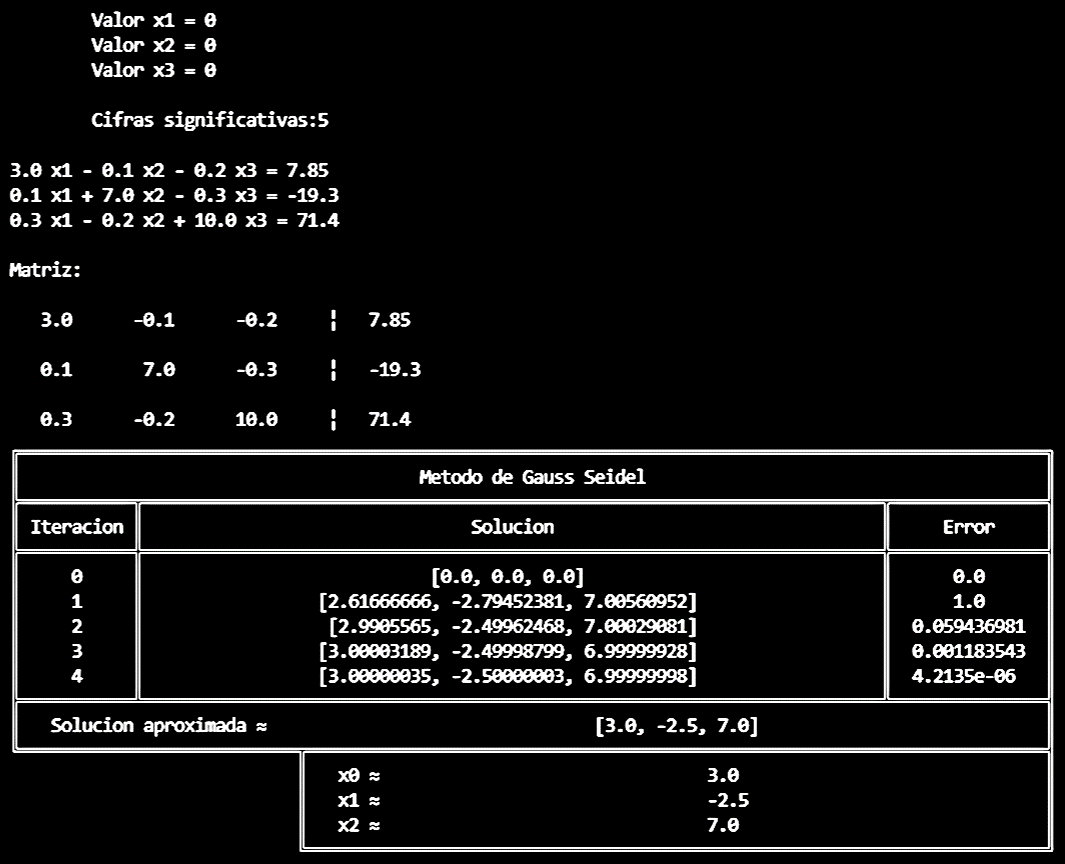
\includegraphics[width=\linewidth]{Figura 1.png}
				Figura 1: Interfas de mi programa despues de realizar las iteraciones para encontra la solucion del sistema anterior, con el metodo de Gauss Seidel.
			\end{center}
			Vemos que mi programa converge en 4 iteraciones y llega a la solución antes dicha, ahora voy a meter un sistema de ecuaciones 
			donde la diagonal no sea dominante, mi programa me arroja lo que se muestra en la figura 2 del sistema de ecuaciones siguiente.
			\begin{align*}
				1x_1 + 2x_2 + 3x_3 &= 4 \\
				5x_1 + 6x_2 + 7x_3 &= 8 \\
				9x_1 + 1x_2 + 2x_3 &= 3
			\end{align*}
			o visto de forma matricial
			$$
			\left(\begin{array}{ccc}
				1 & 2 & 3 \\
				5 & 6 & 7 \\
				9 & 1 & 2
			\end{array}\right)
			\left(\begin{array}{c}
				x_1 \\
				x_2 \\
				x_3 
			\end{array}\right)
			   =
			\left(\begin{array}{c}
			 4 \\
			 8 \\
			 3 
			\end{array}\right)
			$$
			La solución de este sistema es $ x_1 = 0 $, $ x_2 = -1 $ y $ x_3 = 2 $
			\begin{center}
				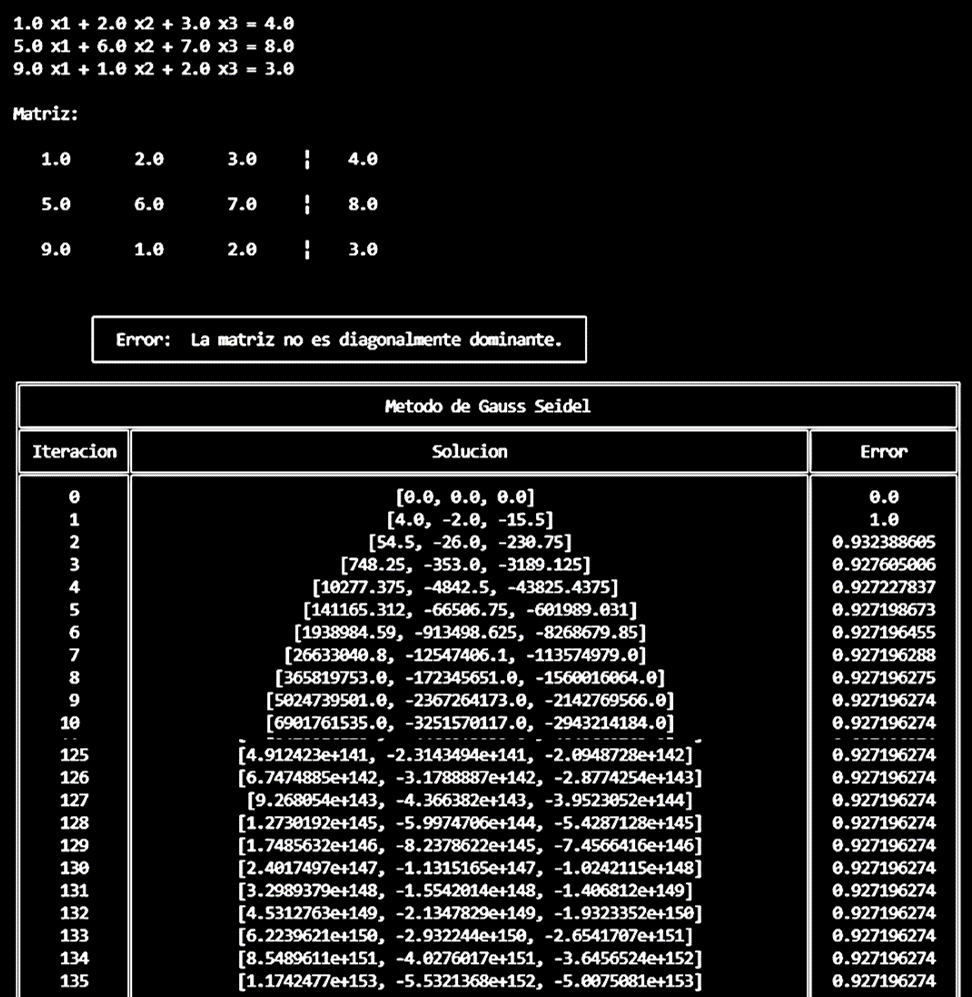
\includegraphics[width=\linewidth]{Figura 2.png}
				Figura 1: Interfas de mi programa despues de realizar las iteraciones para encontra la solucion del sistema con diagonal no dominate, con el metodo de Gauss Seidel.
			\end{center}
			Si vemos la figura 2 podemos ver que mi programa al iterar con un sistema con diagonal no dominante, no encuentra la solución del sistema ya que el método diverge y pues 
			se queda en un ciclo iterando infinitamente sin llegar a la solución.

		\section*{\centering Observación}\label{sec:Observacion}
			En algunas ocasiones, aunque la diagonal no fuera dominante el método si podía aproximaba a 
			la solución del sistema, lo diferencia es que se tardaba más de 20 iteraciones encontrarla o hasta 
			más de 100, pero esto ocurría con muy pocos sistemas con la mayoría que no tenían diagonal 
			dominante no se encontraba la solución.
			En otras ocasiones me encontré con sistemas de ecuaciones que no pueden tener un diagonal 
			dominante, de ninguna forma en la que se acomoden las ecuaciones. \\
			Por todo esto y por las demás condiciones que se necesitan para mi este método es muy 
			deficiente ya que no siempre nos encontramos con un sistema que tenga una diagonal dominante, 
			y hasta hay sistemas que no pueden tener un diagonal dominante. Esto hacer que tenga muchas 
			limitaciones.

		\section*{\centering Conclusión}\label{sec:Conclusion}
			El método de gauss seidel es un método iterativo que tiene como condiciones principales, que el sistema
			tenga una diagonal dominante y que no tenga ceros en la diagonal. Se da un valor inicial a cada 
			variable con el cual se puede iterar. se despeja cada variable en las ecuaciónes y se comienza a 
			obtener el valor de la primera variable con los valores iniciales dados, después se obtiene el valor 
			de la segunda variable con el valor de la variable anterior obtenida y con los valores iniciales 
			dados, y así sucesivamente hasta encontrar la solución del sistema. Cuando la diagonal no es 
			dominante en ocasiones si encuentra la solución, pero la mayoría de las veces no, sé queda en un 
			ciclo infinito, y si encuentra la solución hace mucha iteración.

		\centering
		\begin{thebibliography}{10}
			\bibitem{bib:item1} Luis, V. (2021). Métodos numéricos para la física y la ingeniería. En Métodos iterativos (Primera ed., pp. 135–140). DERECHOS RESERVADOS.
			\bibitem{bib:item2} Federico, D. S. C., \& Antonio, N. H. (2014). Métodos Numéricos Aplicados a la Ingeniería. En Métodos iterativos (pp. 231–242). Grupo Editorial Patria.
			\bibitem{bib:item3} Steven, C. C., \& P. C. Raymond (2006). Metodos Numericos Para Ingenieros, Matrices especiales y el método de Gauss-Seidel, GAUSS-SEIDEL (Quinta ed., pp. 310–317). McGRAW-HILL/INTERAMERICANA EDITORES.
		\end{thebibliography}

	\end{document}